\section{Introduction}
At first glance, recording images from hardware synchronized cameras seems a
trivial task. After all, the cameras are already synchronized, so
where is the problem?

Indeed this is straight forward when running at low frame rates over
an under utilized, reliable, low latency link such as e.g. USB3. Then
frames that are triggered by the same sync pulse will arrive as a
batch, and a simple algorithm that groups frame by time proximity will work.

Things however become tricky if for instance the receiving host has
significant CPU load that will induce occasional delays in frame arrival
times. Even more difficult are IP cameras, in particular if they are
operated at frame rates that are close to saturating the bandwidth of
the network link. Then, frames may arrive late by well more
than 1/2 of a frame period, or may be dropped at the network level
altogether. Arrival times are also affected when exposure times are
adjusted independently across cameras, compounding the problem.

Fig. \ref{fig:perioddist} shows the distribution of frame periods,
i.e. the time elapsed between consecutive frames from a single camera,
divided by the actual frame period of 25ms. While most frames are
spaced by about 25ms as expected, about 21\% arrive early or late by more than 1/2 a frame
period, and as such would be assigned incorrectly by naive time
proximity grouping.
\begin{figure}[h]
	\centering
	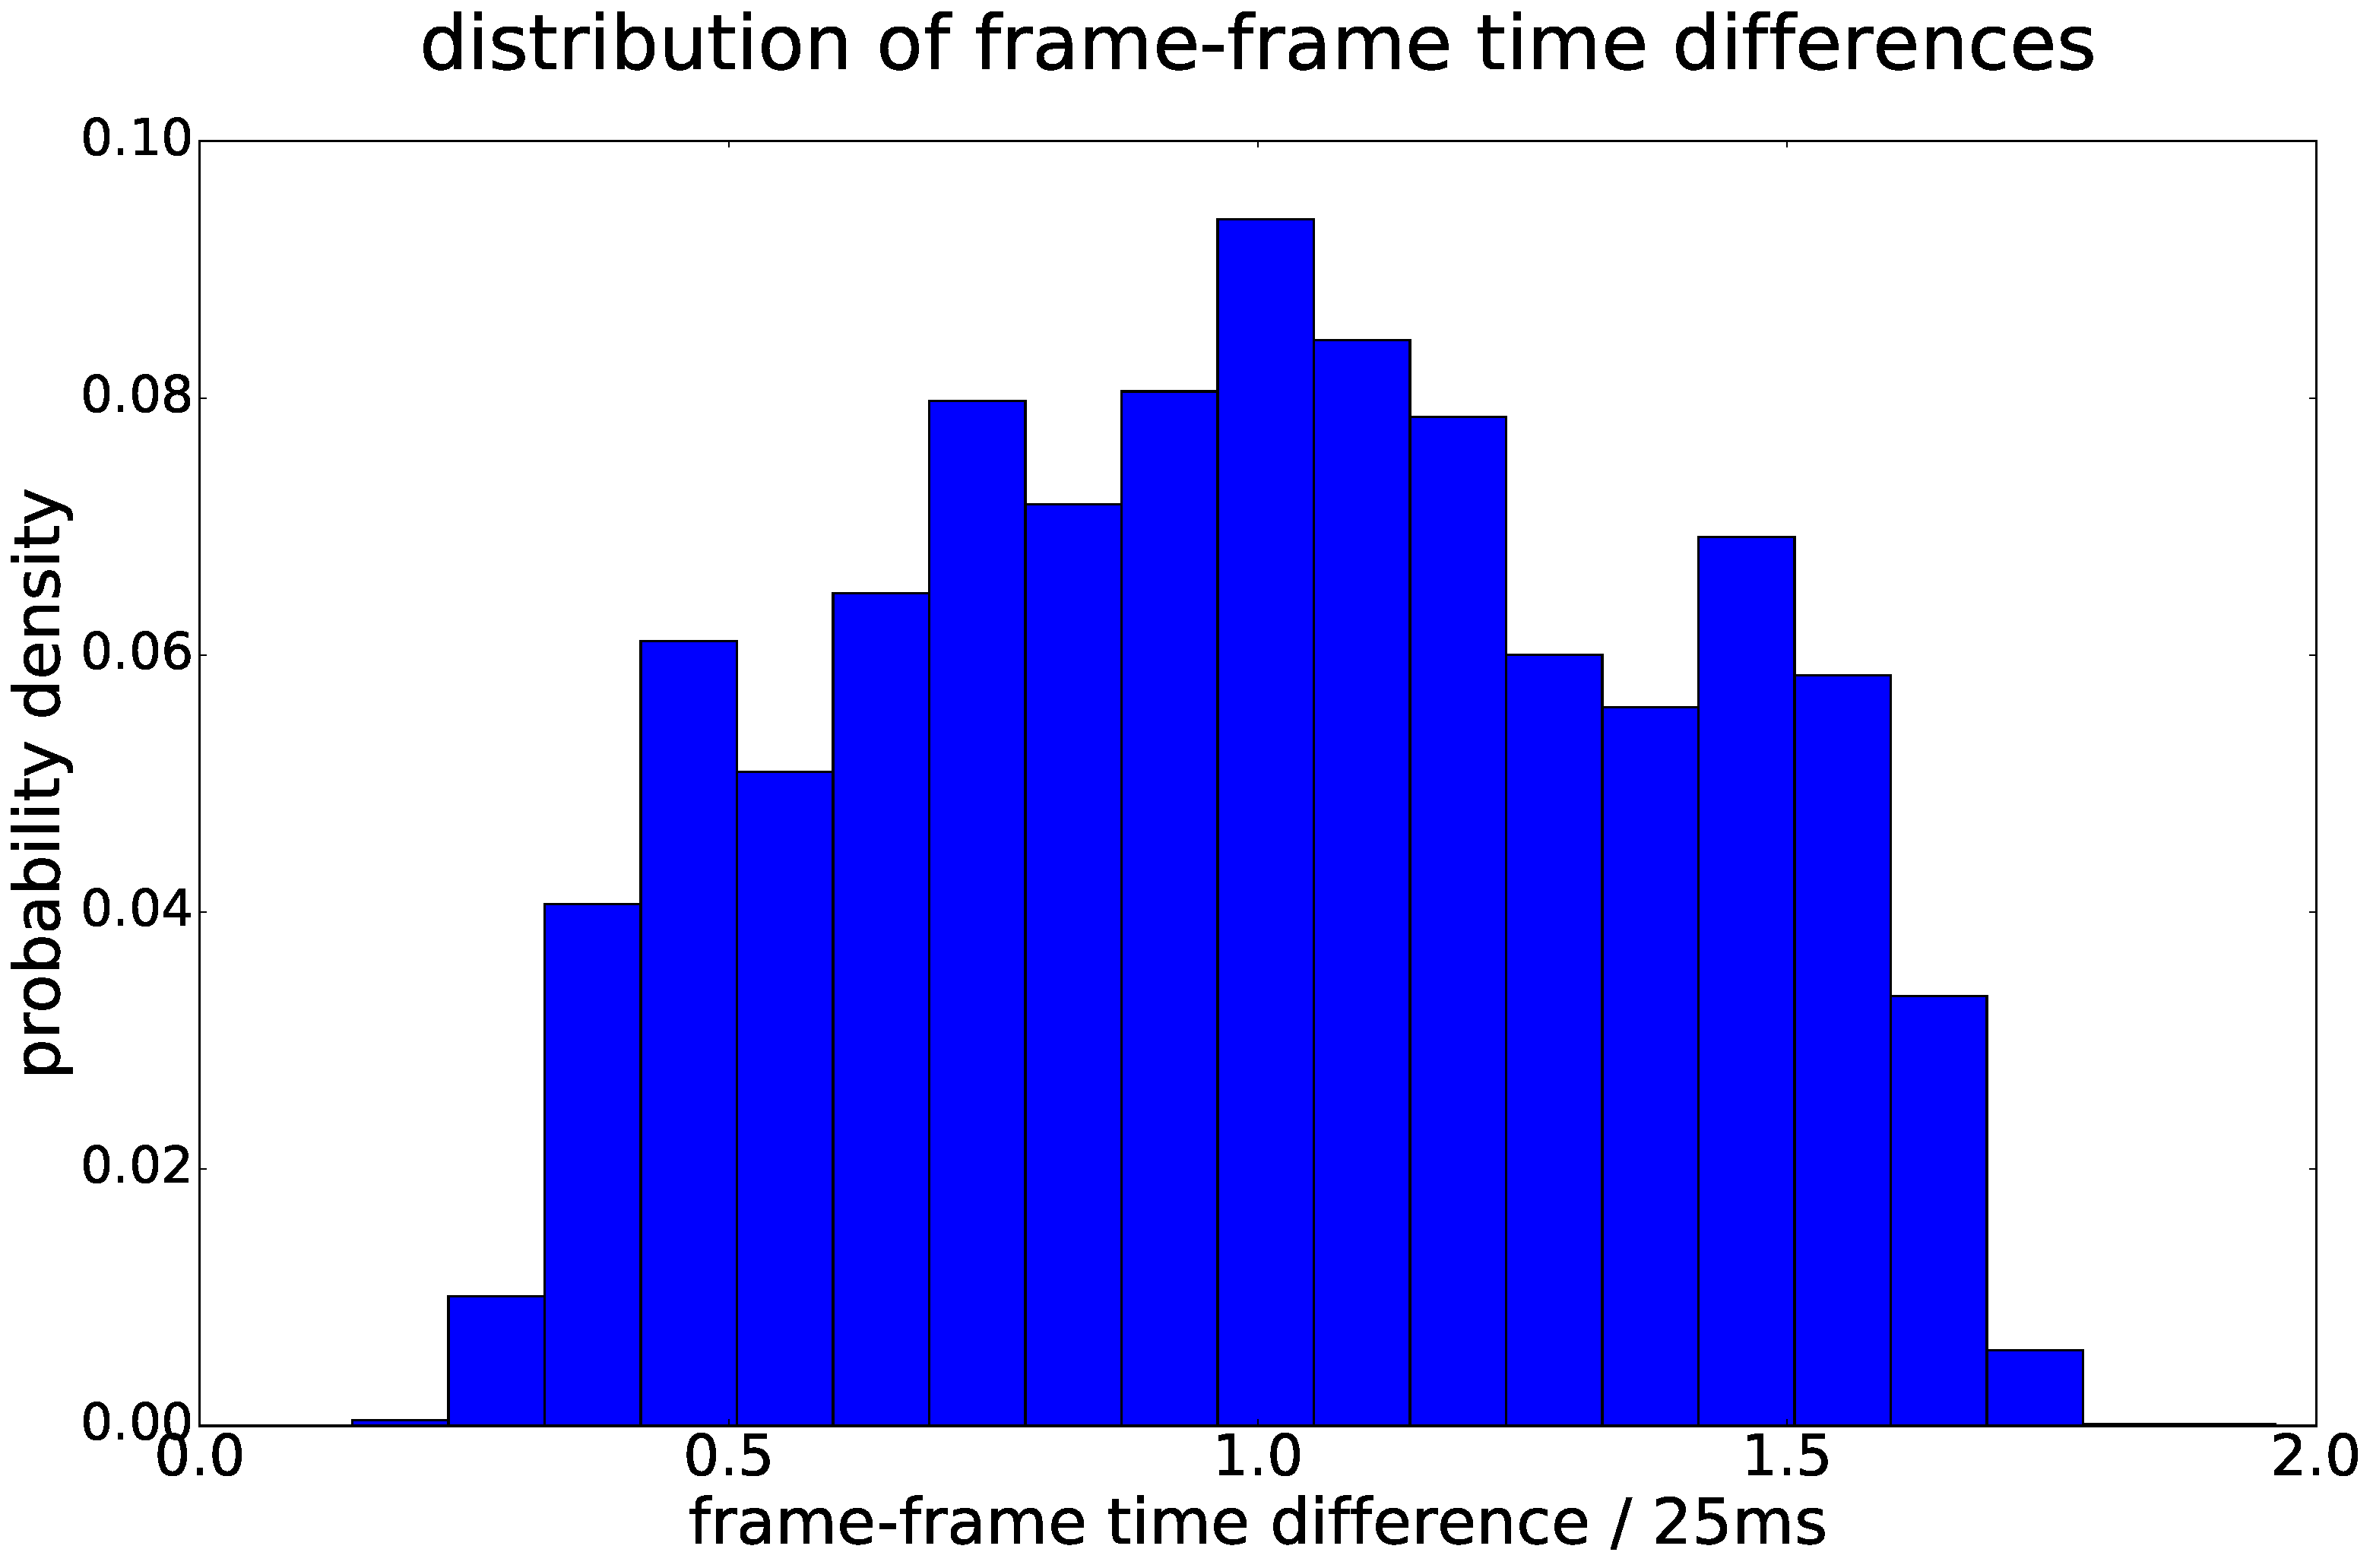
\includegraphics[width=\linewidth]{figures/period_dist.pdf}
        \caption{Distribution of frame periods, i.e. frame-to-frame time arrival
          differences for a single camera. The times have been divided
          by the sync pulse period of 25ms, such that a value of 1
          along the x axis corresponds to two frames that have arrived
          exactly  25ms apart.}
    \label{fig:perioddist}
\end{figure}

Fig. \ref{fig:arrival_vs_frame} illustrates this more clearly. Along
the $x$ axis it shows the ``true'' frame time $T$ (more about this in
section \ref{sec:sync_algo}), along the $y$ axis the actual time the
corresponding images arrived at the host. One can see that by the time
the last image corresponding to one sync pulse arrives, the first one
for the next sync pulse follows right
away. In Fig. \ref{fig:arrival_vs_frame}, all arrival time stamps have
been aggregated into a vertical line at time stamp 137.85s to
demonstrate how difficult it is to recover frame boundaries just by
looking at arrival time stamps.
\begin{figure}[h]
	\centering
	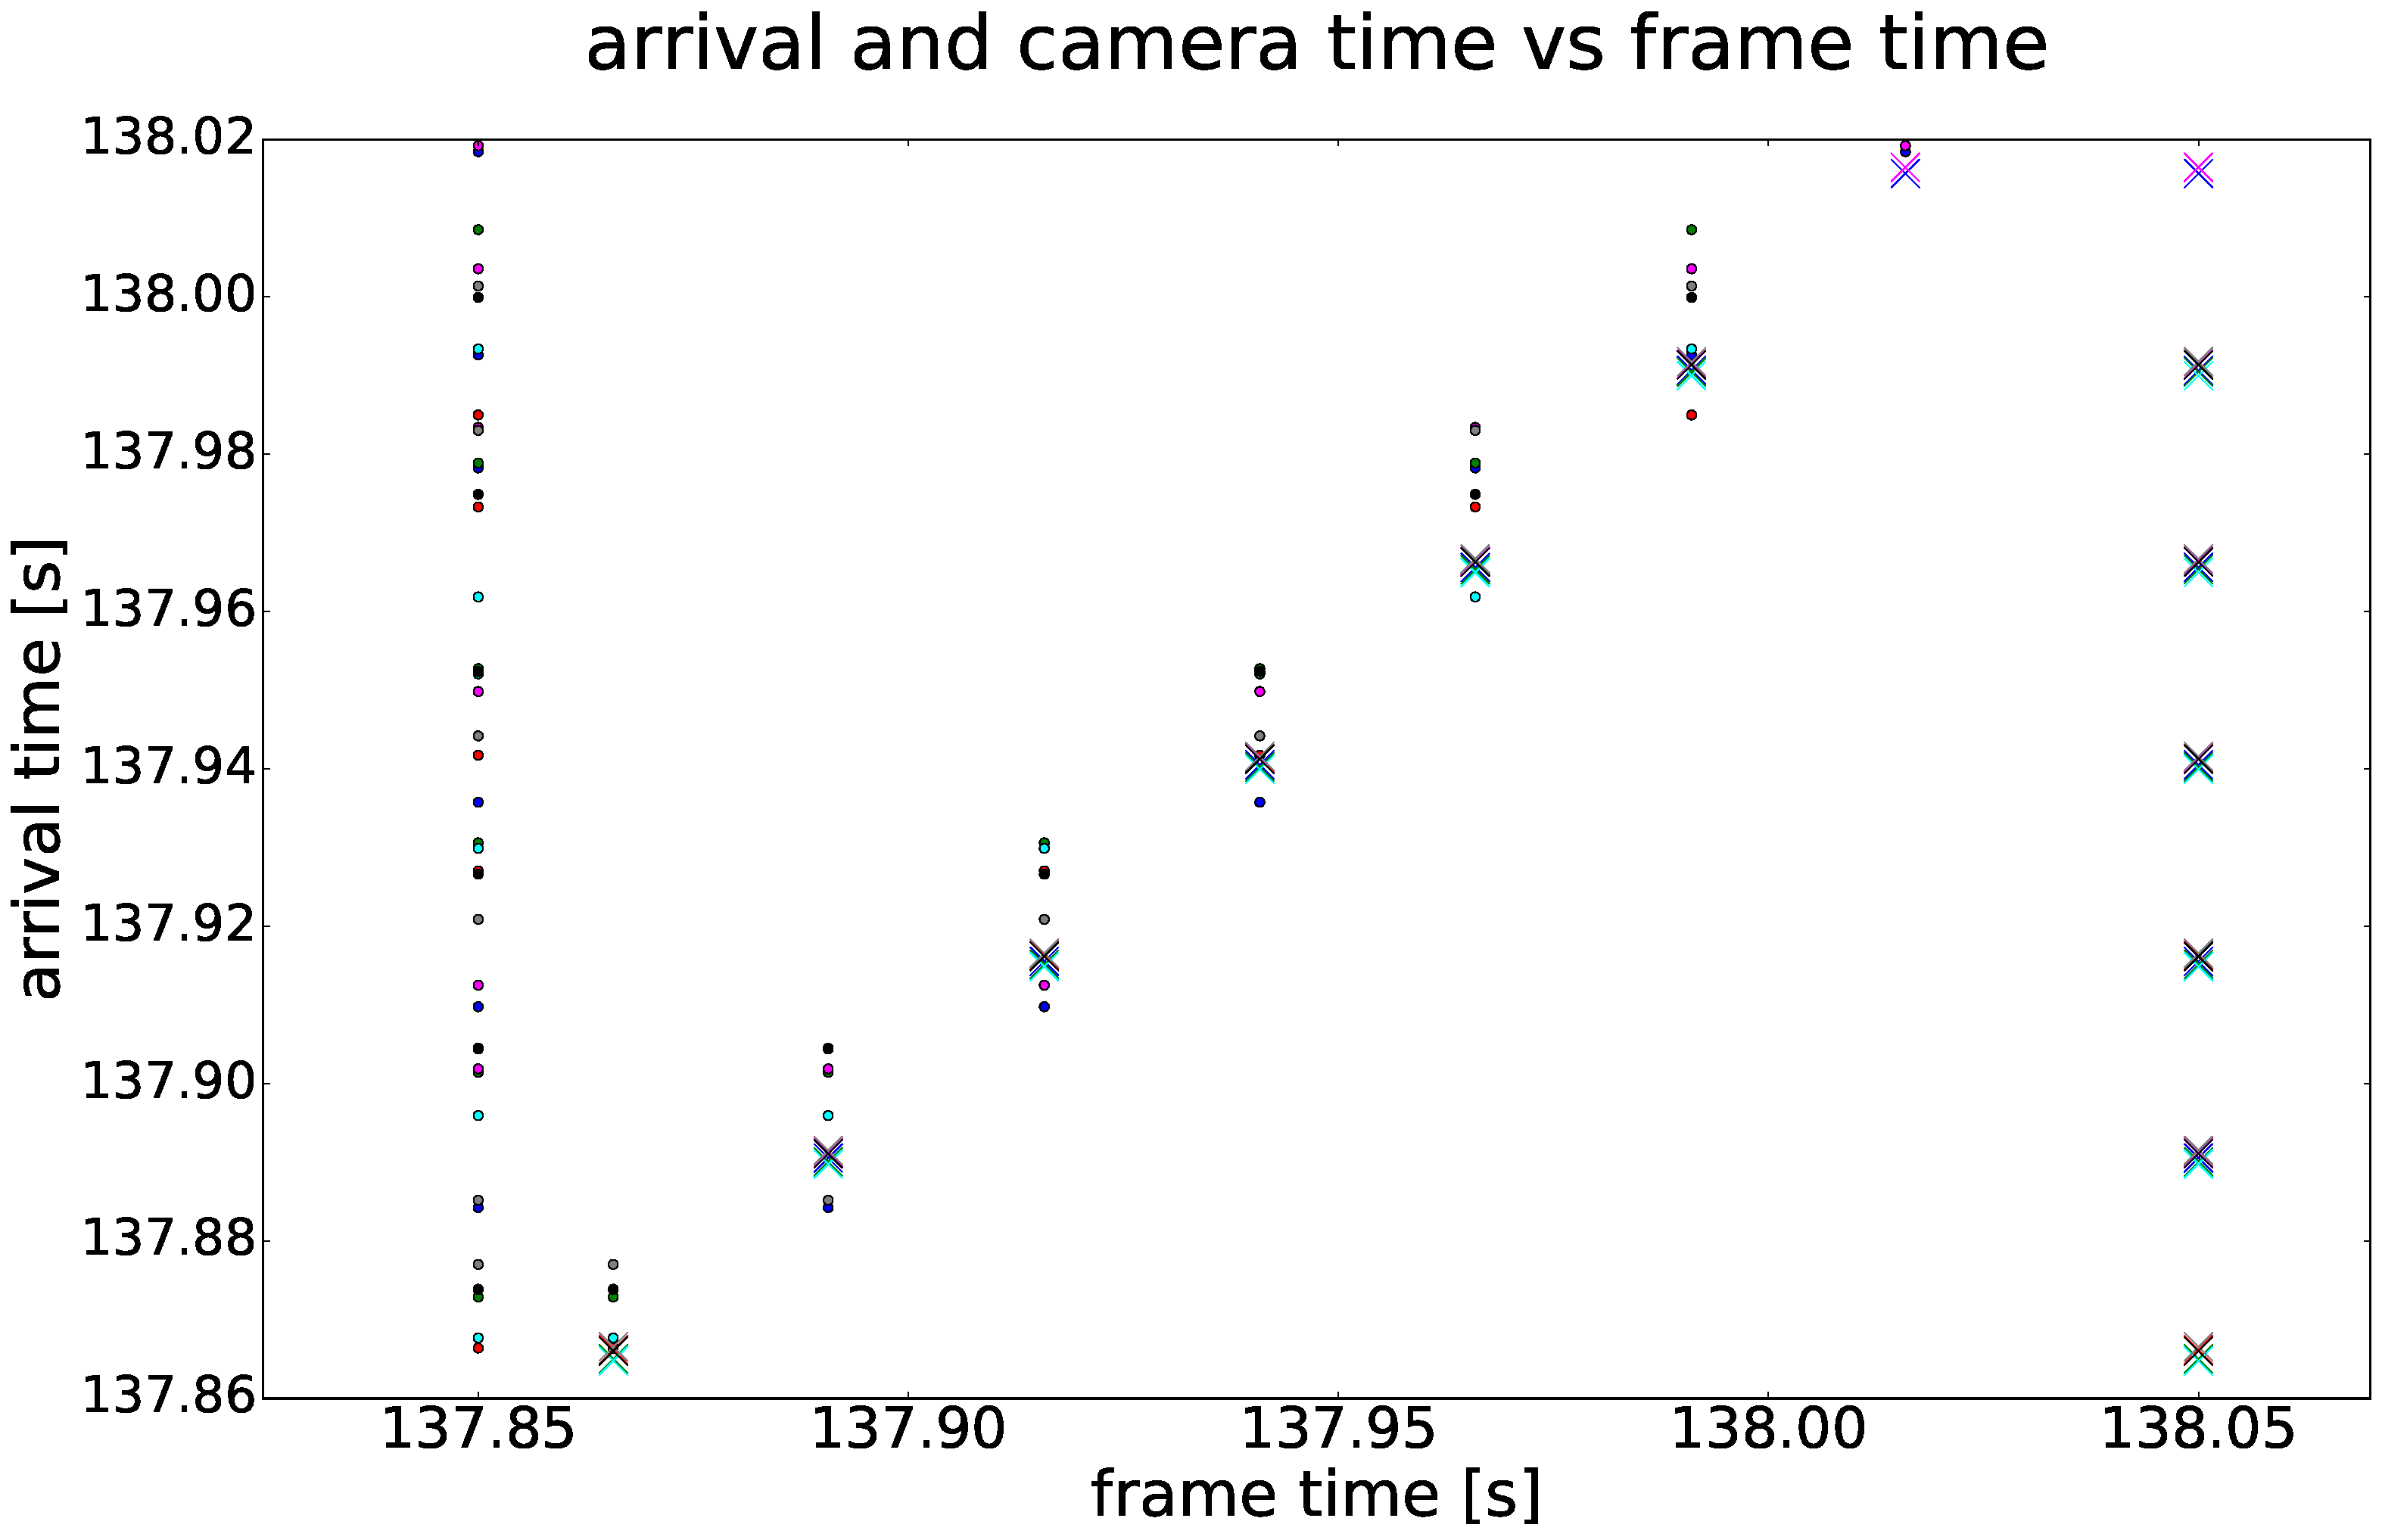
\includegraphics[width=\linewidth]{figures/arrival_vs_frame.pdf}
        \caption{
          Time of arrival $\atime{}$, filled circles, and
          camera time, $\ttime{}$, crosses, plotted vs the sync pulse
          time $T$. The color indicates the camera index $i$. To
          visualize how challenging it is to group frames based on
          arrival time only, all arrival times have been collapsed onto a
          single frame at $T$=137.85s. Grouping by the filtered camera
          time $\ttime{}$ however is straight forward, as is shown at $T$=138.05s.}
    \label{fig:arrival_vs_frame}
\end{figure}

Fortunately many computer vision cameras offer the option to embed 
camera time stamps right at the imager, before the frame is sent over
the wire. Although the clocks on the cameras are offset with
respect to each other, and will drift over time, they provide a way to
reliably detect dropped frames, which is crucial for removing jitter
from the arrival times.

After several failed attempts, we eventually found a robust method
of assigning time stamps to frames. Moreover, our method has good diagnostic
capabilities and reliably produces alerts when synchronization is no
longer possible due to e.g. failed 
hardware synchronization or excessive CPU load.

This paper documents the lessons learned during the
implementation. The method described here is implemented in the ROS
\cite{ros} ``CamSync'' node, which we hope will be useful for other projects
that require accurate synchronized timestamps in a multi-camera
setting. The code can be found at
\href{https://github.com/daniilidis-group/cam_sync}{https://github.com/daniilidis-group/cam\_sync}.
